\chapter{Building Block View Static View}

\section{Overview}
\RequirementTag{SDD_PNC}{034}

SUM_PNC manages all of the BSW services related to Partial Networks (PNs) for an ECU that is a member of any PN. SUM_PNC shall be implemented in all ECUs that are members of any PN. This allows all other SW-Cs to function abstracted from the source of the data (e.g. signals deployed to the serial communication networks).

Actions under taken in order to accomplish system goals, PNC shall, 

\begin{enumerate}[label=\roman*.]
	\item Request to BswM to activate / deactivate PN per the activation / deactivation criteria.
	\item Publish notification that can be used by SW-Cs that participate in the PN, to know when the infrastructure services are ready to transmit and receive signals;
	\item Perform retries for PN activation / deactivation requests.
	\item SUM\_PNC shall contain logic to compare the status of the Mode Request port interface to BswM with the corresponding Mode User port interface. SUM\_PNC needs to make sure that the BSW state matches the requested state. SUM\_PNC logic requests for PN activation needs to be in sync with the actual BSW PN activation status.
	\item SW-C which sends signals via serial data communication shall use the appropriate return codes from the AUTOSAR communication / RTE layer to confirm transmission.
\end{enumerate}

{\Satisfies{SRS\_PNC 003} \Satisfies{SRS\_PNC 005} \Satisfies{SRS\_PNC 023} \Satisfies{SRS\_PNC 043}}

The following diagram shows the main building blocks of the system.
The interfaces and dependent SUMs, BSW modules are described in below.

\begin{figure}[h!]
	\centering
	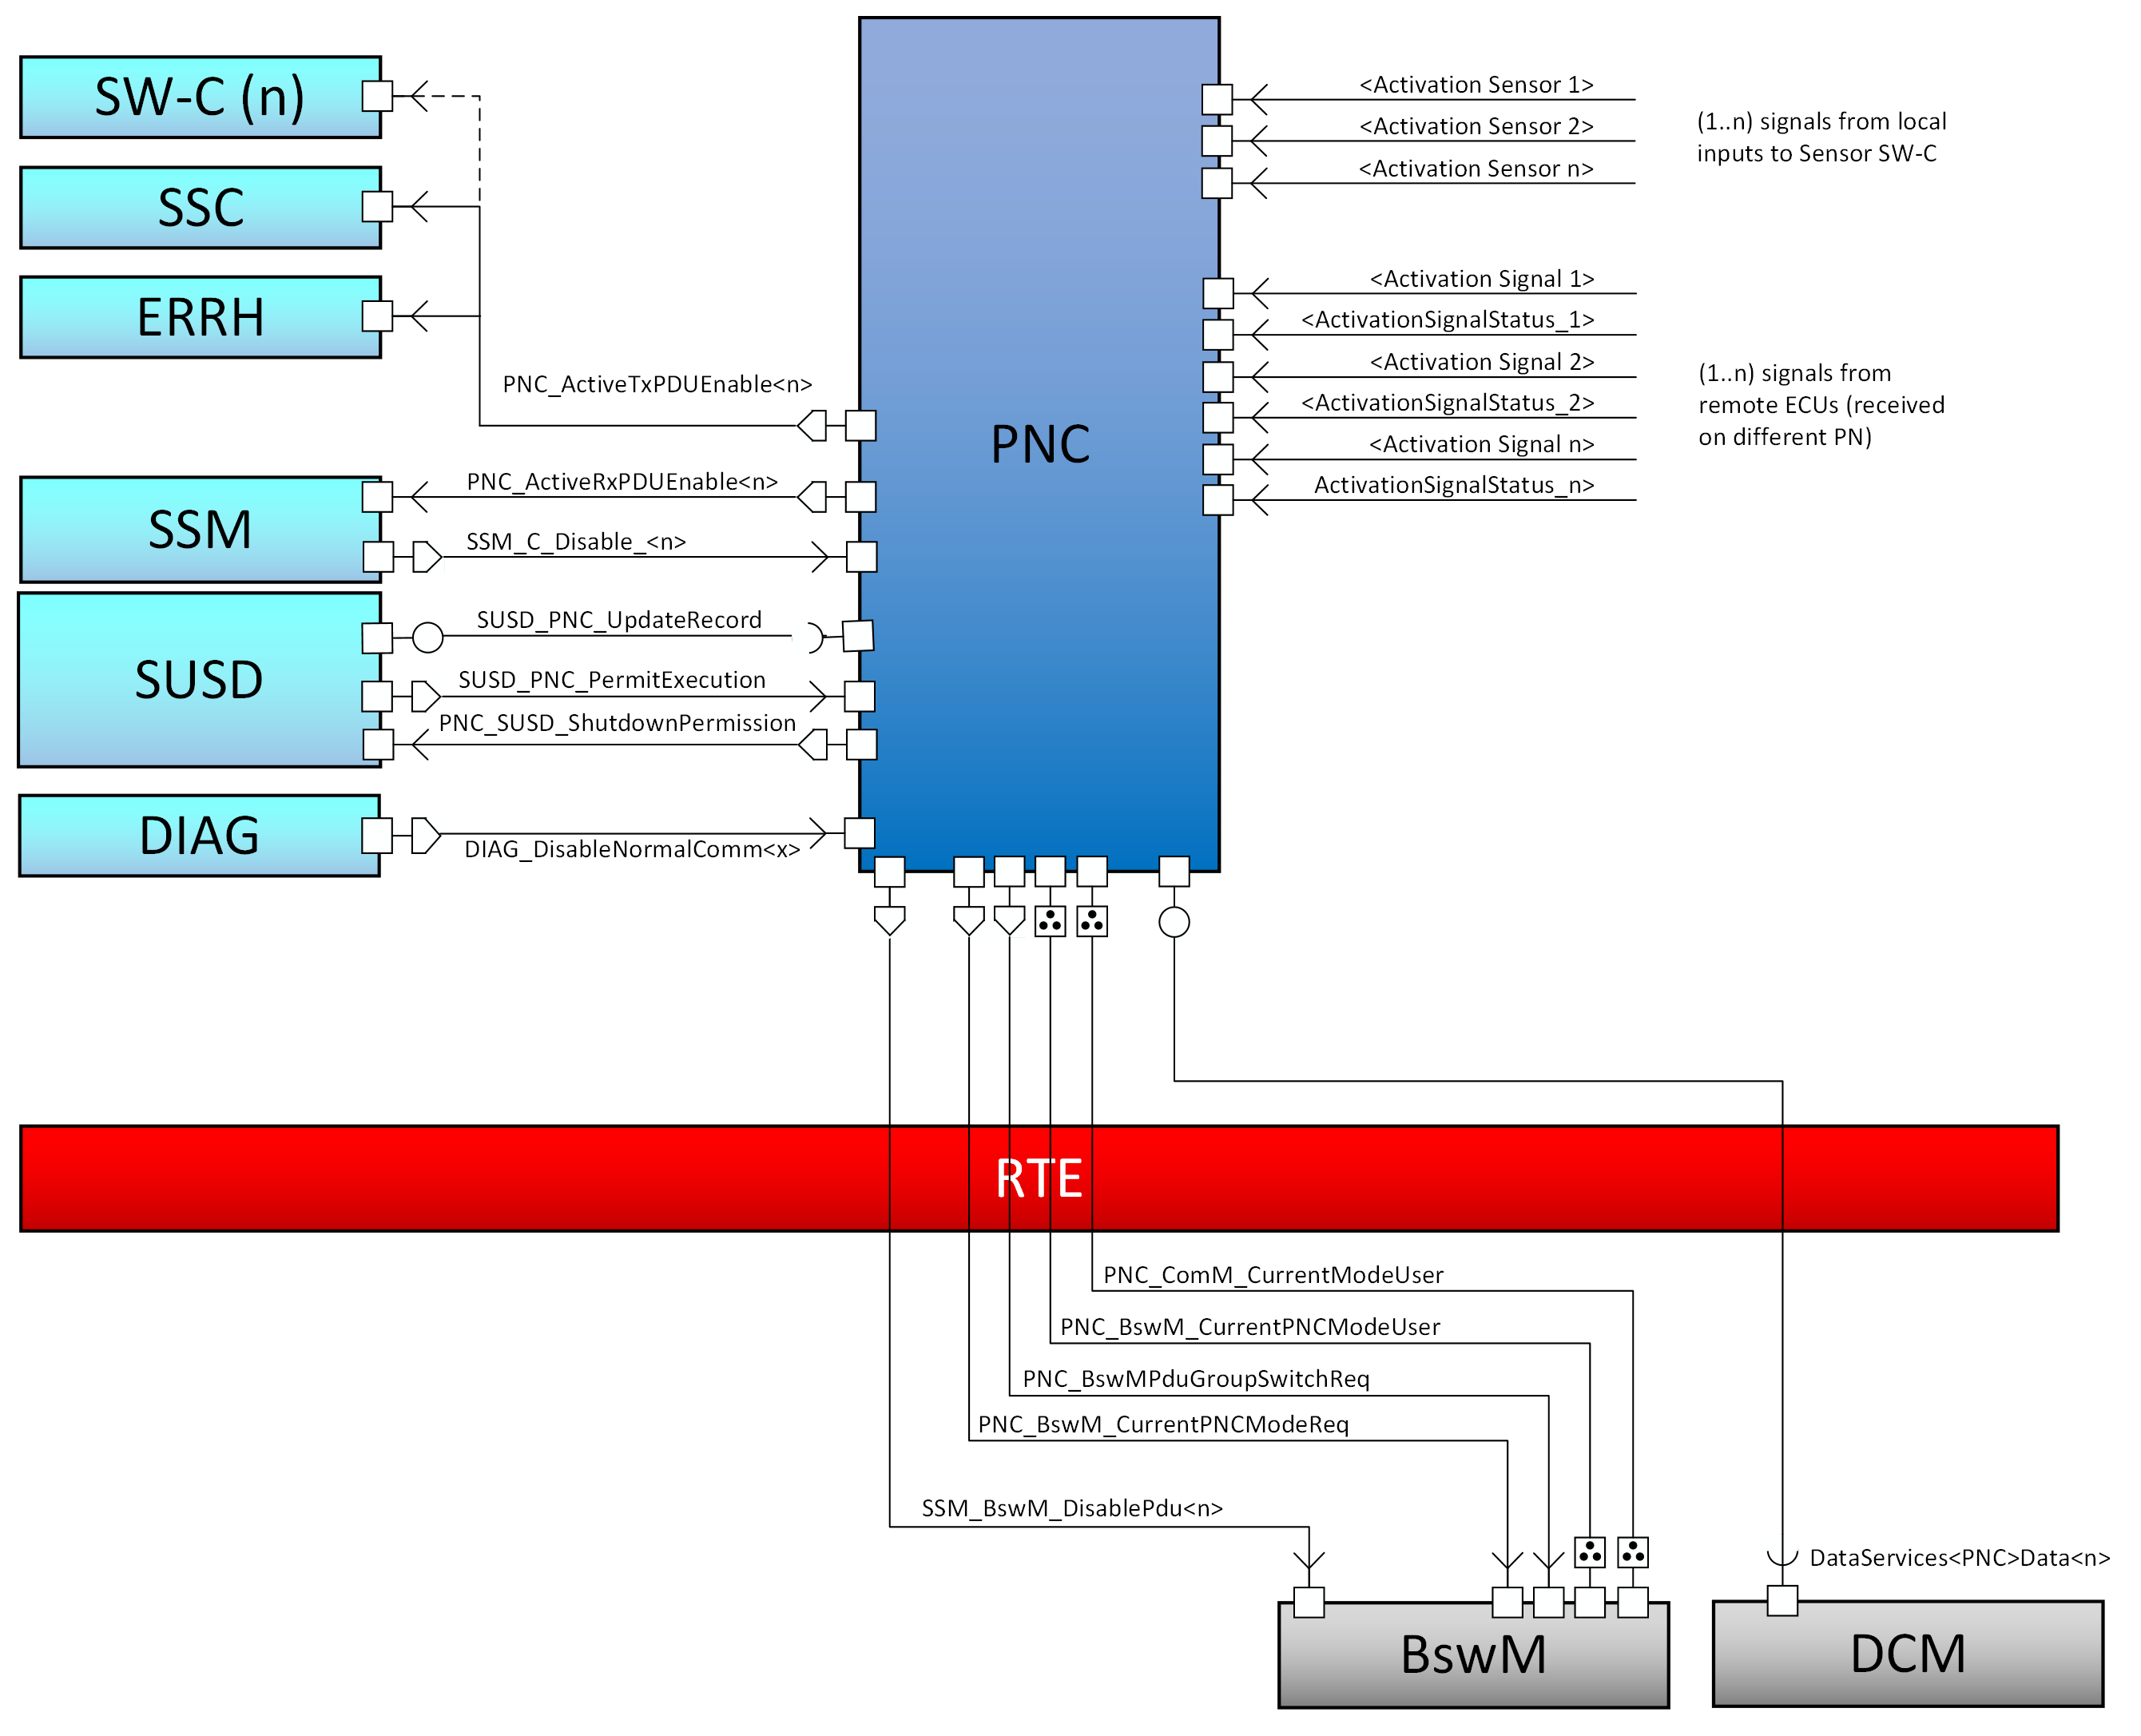
\includegraphics[scale=0.65]{images/blockDiagIF.png}
	\caption{SUM\_PNC Interfaces representation}
\end{figure}

\subsection{SUM\_SUSD}
\label{subsection:SumSusd}
\RequirementTag{SDD_PNC}{002}

Dependency and purpose of this module wrt PNC is mentioned below:

\begin{itemize}
\item The Standard Utility Module, Startup Shutdown (SUM\_SUSD) contains the following functions: Application State Manager, Application SW-C Start /Shutdown, Operating/Battery Voltage Monitor, and Wakeup Reason DID.
\item SUM\_SUSD shall set the Wakeup(s) Active bit in the SUSD\_PNC\_PermitExecution interface to SUM\_PNC to:
\begin{itemize}
	\item FALSE - when no wakeups relevant to PN activation are active
	\item TRUE - when any wakeup(s) relevant to PN activation are active
\end{itemize}
\item SUM\_SUSD shall set the HW Ready bit in the SUSD\_PNC\_PermitExecution interface to SUM\_PNC to:
\begin{itemize}
	\item FALSE - when Project Specific HW needed for PN activation is not ready
	\item TRUE - when Project Specific HW needed for PN activation is ready
\end{itemize}
\item PNC shall publish Signal PNC\_ShutdownPermission to SUM\_SUSD to inform if any PN is currently active or not.
\end{itemize}
\begin{itemize}
    \item The PNC shall utilize the \code{SUSD\_PNC\_UpdateRecord} interface to notify the SUSD of the activation or deactivation of a PN, specifying the type (local/remote) and the reason for the activation.
    \item The Record ID (\code{RID\_Enum}) values used in this notification are derived from the SPM record identification scheme: \code{SPM\_PNC\_LOC\_DIAG\_RID} (0x25) for the aggregated locally active PN view, and \code{SPM\_PNC\_REMOTE\_RID} (0x02) for the aggregated remotely active PN view.
    \item The wakeup reason (\code{RWR} field of \code{RecordIdType}) is the \code{PartialNetworkName} value of the primary activating PN. For local activation this is the first active source in the per-PN history buffer; for remote activation this is the minimum active PN name from the NM activation list.
\end{itemize}

{\Satisfies{SRS\_PNC 013} \Satisfies{SRS\_PNC 008} \Satisfies{SRS\_PNC 010} \Satisfies{SRS\_PNC 011} \Satisfies{SRS\_PNC 107} \Satisfies{SRS\_PNC 108}}


\subsection{SUM\_DIAG}
\RequirementTag{SDD_PNC}{003}

Dependency and purpose of this module wrt PNC is mentioned below:

\begin{itemize}
	\item The Standard Utility Module, Diagnostic Application Service (SUM\_DIAG), Preconditions to support diagnostic ECU Reset service, Preconditions to support Communication Control service request etc.
    \item SUM\_DIAG provides notification about the status of diagnostics enabling or disabling of normal communications for each $<$channel$>$ to PNC.
    \item SUM\_PNC shall check disable normal communication from the tester to inhibit remote activation of a PN if not yet active as Passive ECUs do not need to remotely activate a PN when normal communication is disabled.
\end{itemize}

{\Satisfies{SRS\_PNC 025}}

\subsection{SUM\_SSFM}
\RequirementTag{SDD_PNC}{035}
\\
Dependency and purpose of this module wrt PNC is mentioned below:

\begin{itemize}
\item Part of the Standard Utility Module Signal Status and Fault Monitor (SUM\_SSFM)’s scope is for handling status information related to the Signal Integrity and Source Integrity for received signals, and for handling of generating/checking safety signal transmitted/received with in a protected signal group.

\item SUM\_PNC shall publish Signal PNC\_ActiveRxPDUEnable$<$n$>$\_Enable to SUM\_SSFM to notify PN$<$n$>$ rx status (enabled / disabled).

\item SUM\_SSFM shall transit to SIG\_STATUS\_DISABLED by use of the appropriate SUM\_PNC notification, PNC\_SWC\_PN$<$n$>$Enable, to be notified when all partial networks for the associated signal are inactive
\Satisfies{SRS\_PNC 026}

\item SUM\_PNC shall publish PN\_DTC\_Allowed$<$n$>$ to SUM\_SSFM so that SUM\_SSFM updates the PN\_DTC\_Enabled Flags related to Loss of Comm or Invalid Data DTCs.

\end{itemize}

\subsection{SUM\_SOH}
Dependency and purpose of this module wrt PNC is mentioned below:

\begin{itemize}
	\item The Standard Utility Module, State of Health manager (SUM\_SOH) contains the following functions: Aggregation/Monitoring of SW platform modes (BSW States), WdgM SE states, reset requests and their occurrences.
	\item SUM\_PNC shall publish Signal PNC\_ActiveTxPDUEnable<n> to SUM\_SOH, that PN<n> failed attempt to start
	\item SUM\_SOH shall only publish the reliability monitor events signal when the PNC\_ActiveTxPDUEnable interface is TRUE. If the PNC\_ActiveTxPDUEnable interface is FALSE, then SOH shall retain the reliability monitor events signal in its output buffer.
\end{itemize}

\subsection{SUM\_ERRH}
Dependency and purpose of this module wrt PNC is mentioned below:

\begin{itemize}
	\item The Standard Utility Module, Error Handler (SUM\_ERRH), is notified of error events created by BSW Production Errors or SUM error events;
	\item SUM\_ERRH shall implement a port, PNC\_ActiveTxPDUEnable, to receive notification of the availability of the Partial Network in which the message containing the DTC Triggered signal group participates;
	\item SUM\_ERRH shall only publish the DTC Triggered signal when PNC\_ActiveTxPDUEnable is TRUE. If PNC\_ActiveTxPDUEnable is FALSE, then SUM\_ERRH shall retain the DTC Triggered message in its output buffer;
	\item SUM\_PNC shall publish Signal PNC\_ActiveTxPDUEnable<n> to SUM\_SSC, SUM\_SOH, and SUM\_ERRH. Publish notification to notify PN<n> tx status (enabled / disabled).
\end{itemize}

\subsection{SUM\_SSC}
\RequirementTag{SDD\_PNC}{006}
\\
Dependency and purpose of this module wrt PNC is mentioned below:

\begin{itemize}
	\item The Standard Utility Module, Security Service Coordinator (SUM\_SSC), is responsible for functions like Transmitter of authenticated messages, transmitter of non-authenticated messages having ARC, PV, CS/CSR etc.
	\item SUM\_PNC shall publish Signal PNC\_ActiveTxPDUEnable<n> to SUM\_SSC, to notify PN<n> tx status (enabled / disabled).\\
\Satisfies{SRS\_PNC 026}
    \item SUM\_PNC shall publish PN\_DTC\_Allowed<n> to SUM\_SSC so that SUM\_SSC updates the PN\_DTC\_Enabled Flags related to the U1962 DTC.
\end{itemize}

\subsection{BSW Elements: System, Services}
\RequirementTag{SDD\_PNC}{043}
\\
\subsubsection{\textit{BswM}}
\begin{itemize}
	\item AUTOSAR Basic Software module BSW Mode Manager (BswM), Its responsibility is to arbitrate mode requests from application layer SW-Cs or other BSW modules based on simple rules, and perform actions based on the arbitration result.
	\item SUM PNC shall have mode requester interface and mode switch interface to get information on Current PNC mode, request to enable/disable relevant Tx/Rx group.
	
	\begin{longtable}{|l|l|l|}
\hline
\begin{minipage}{0.38\linewidth}\raggedright\vspace{.75ex}{\cellcolor{eTASPurple}\textcolor{white}{\bfseries Mode Requester interface (PNC-BSWM)} }\vspace{.75ex}\end{minipage} & \begin{minipage}{0.38\linewidth}\raggedright\vspace{.75ex}{\cellcolor{eTASPurple}\textcolor{white}{\bfseries Description} }\vspace{.75ex}\end{minipage} & \begin{minipage}{0.15\linewidth}\raggedright\vspace{.75ex}{\cellcolor{eTASPurple}\textcolor{white}{\bfseries  Info obtained via} }\vspace{.75ex}\end{minipage}\\
\hline\hline
\endfirsthead
\hline
\begin{minipage}{0.38\linewidth}\raggedright\vspace{.75ex}{\cellcolor{eTASPurple}\textcolor{white}{\bfseries Mode Requester interface (PNC-BSWM)} }\vspace{.75ex}\end{minipage} & \begin{minipage}{0.38\linewidth}\raggedright\vspace{.75ex}{\cellcolor{eTASPurple}\textcolor{white}{\bfseries Description} }\vspace{.75ex}\end{minipage} & \begin{minipage}{0.15\linewidth}\raggedright\vspace{.75ex}{\cellcolor{eTASPurple}\textcolor{white}{\bfseries  Info obtained via} }\vspace{.75ex}\end{minipage}\\
\hline\hline
\endhead
\hline
\endfoot
\hline
\endlastfoot
\begin{minipage}{0.38\linewidth}\raggedright\vspace{.75ex}{\cellcolor{eTASGray30} PNC\_BswM\_CurrentPNCModeReq}\vspace{.75ex}\end{minipage} & \begin{minipage}{0.38\linewidth}\raggedright\vspace{.75ex}{\cellcolor{eTASGray30} PNC\_BswM\_CurrentPNCModeReq to request the appropriate PN(s) to be activated / deactivated}\vspace{.75ex}\end{minipage} & \begin{minipage}{0.15\linewidth}\raggedright\vspace{.75ex}{\cellcolor{eTASGray30} ComM}\vspace{.75ex}\end{minipage}\\\hline
\begin{minipage}{0.38\linewidth}\raggedright\vspace{.75ex}{\cellcolor{eTASGray30} PNC\_BswMPduGroupSwitchTxReq}\vspace{.75ex}\end{minipage} & \begin{minipage}{0.38\linewidth}\raggedright\vspace{.75ex}{\cellcolor{eTASGray30}  To request enabling / disabling relevant Tx PDU groups}\vspace{.75ex}\end{minipage} & \begin{minipage}{0.15\linewidth}\raggedright\vspace{.75ex}{\cellcolor{eTASGray30} Com}\vspace{.75ex}\end{minipage}\\\hline
\begin{minipage}{0.38\linewidth}\raggedright\vspace{.75ex}{\cellcolor{eTASGray30} PNC\_BswMPduGroupSwitchRxReq}\vspace{.75ex}\end{minipage} & \begin{minipage}{0.38\linewidth}\raggedright\vspace{.75ex}{\cellcolor{eTASGray30}  To request enabling / disabling relevant Rx PDU groups}\vspace{.75ex}\end{minipage} & \begin{minipage}{0.15\linewidth}\raggedright\vspace{.75ex}{\cellcolor{eTASGray30} Com}\vspace{.75ex}\end{minipage}\\\hline
\begin{minipage}{0.38\linewidth}\raggedright\vspace{.75ex}{\cellcolor{eTASGray30} PNC\_BswM\_PDUGroup\_DM\_Switch}\vspace{.75ex}\end{minipage} & \begin{minipage}{0.38\linewidth}\raggedright\vspace{.75ex}{\cellcolor{eTASGray30}  To request enabling / disabling of Rx PDU Group deadline monitoring}\vspace{.75ex}\end{minipage} & \begin{minipage}{0.15\linewidth}\raggedright\vspace{.75ex}{\cellcolor{eTASGray30} Com}\vspace{.75ex}\end{minipage}\\\hline
\end{longtable}
	\begin{longtable}{|l|l|l|}
\hline
\begin{minipage}{0.38\linewidth}\raggedright\vspace{.75ex}{\cellcolor{eTASPurple}\textcolor{white}{\bfseries Mode User interface(PNC-BSWM)} }\vspace{.75ex}\end{minipage} & \begin{minipage}{0.38\linewidth}\raggedright\vspace{.75ex}{\cellcolor{eTASPurple}\textcolor{white}{\bfseries Description} }\vspace{.75ex}\end{minipage} & \begin{minipage}{0.15\linewidth}\raggedright\vspace{.75ex}{\cellcolor{eTASPurple}\textcolor{white}{\bfseries Info obtained via} }\vspace{.75ex}\end{minipage}\\
\hline\hline
\endfirsthead
\hline
\begin{minipage}{0.38\linewidth}\raggedright\vspace{.75ex}{\cellcolor{eTASPurple}\textcolor{white}{\bfseries Mode User interface(PNC-BSWM)} }\vspace{.75ex}\end{minipage} & \begin{minipage}{0.38\linewidth}\raggedright\vspace{.75ex}{\cellcolor{eTASPurple}\textcolor{white}{\bfseries Description} }\vspace{.75ex}\end{minipage} & \begin{minipage}{0.15\linewidth}\raggedright\vspace{.75ex}{\cellcolor{eTASPurple}\textcolor{white}{\bfseries Info obtained via} }\vspace{.75ex}\end{minipage}\\
\hline\hline
\endhead
\hline
\endfoot
\hline
\endlastfoot
\begin{minipage}{0.38\linewidth}\raggedright\vspace{.75ex}{\cellcolor{eTASGray30} PNC\_BswM\_CurrentPNCModeUser}\vspace{.75ex}\end{minipage} & \begin{minipage}{0.38\linewidth}\raggedright\vspace{.75ex}{\cellcolor{eTASGray30}  To inform the current state of the PN}\vspace{.75ex}\end{minipage} & \begin{minipage}{0.15\linewidth}\raggedright\vspace{.75ex}{\cellcolor{eTASGray30}  ComM}\vspace{.75ex}\end{minipage}\\\hline
\begin{minipage}{0.38\linewidth}\raggedright\vspace{.75ex}{\cellcolor{eTASGray30} PNC\_ComM\_CurrentModeUser}\vspace{.75ex}\end{minipage} & \begin{minipage}{0.38\linewidth}\raggedright\vspace{.75ex}{\cellcolor{eTASGray30}  To inform the current state of channels related to the PN(s) for this ECU}\vspace{.75ex}\end{minipage} & \begin{minipage}{0.15\linewidth}\raggedright\vspace{.75ex}{\cellcolor{eTASGray30}  ComM}\vspace{.75ex}\end{minipage}\\\hline
\end{longtable}
	
	\item Requestor of Partial Network will use following PN states for Mode Requests for function PNC\_BswM\_CurrentPNCModeReq <n>
	\begin{itemize}
		\item [a. ] SUM\_PNC\_NO\_COMMUNICATION
		\item [b. ] SUM\_PNC\_REQUESTED
	\end{itemize}
	\item Mode Switch Interface PNC\_BswM\_CurrentPNCModeUser<n> for individual PN will return the current PN state using all states defined below:
	\begin{enumerate}
		\item [a. ] SUM\_PNC\_NO\_COMMUNICATION
		\item [b. ] SUM\_PNC\_PREPARE\_SLEEP
		\item [c. ] SUM\_PNC\_READY\_SLEEP
		\item [d. ] SUM\_PNC\_REQUESTED
	\end{enumerate}
	\item Mode switch interface PNC\_ComM\_CurrentModeUser <n> to indicate current state of ComM for the desired communication channel. The ComM Channel states are defined as below:
	\begin{enumerate}
		\item [a. ] SUM\_COMM\_NO\_COMMUNICATION
		\item [b. ] SUM\_COMM\_FULL\_COM\_READY\_SLEEP
		\item [c. ] SUM\_COMM\_FULL\_COM\_NETWORK\_REQUESTED
		\item [d. ] SUM\_COMM\_FULL\_COMMUNICATION
		\item [e. ] SUM\_COMM\_SILENT\_COMMUNICATION
	\end{enumerate}
	\item Mode Request Interface PNC\_BswMPduGroupSwitchTxReq<n> and PNC\_BswMPduGroupSwitchRxReq<n> (to Com) to request for Tx or Rx PDU Group enabling associated with specific Partial networks.
	\begin{enumerate}
		\item [a. ] SUM\_PDUGRP\_STOP
		\item [b. ] SUM\_PDUGRP\_START
	\end{enumerate}	
	\item Mode Request Interface PNC\_BswM\_PDUGroup\_DM\_Switch<n> to request enabling or disabling the deadline monitoring for the Rx PDU group of the selected PN:
	\begin{enumerate}
		\item [a. ] PN\_DM\_ENABLE
		\item [b. ] PN\_DM\_DISABLE
	\end{enumerate}	
\end{itemize}

\subsubsection{\textit{ComM}}

\begin{enumerate}
	\item The ComM module collects the bus communication access requests from communication requestors and coordinates the bus communication access requests.
	\item ComM updates SUM PNC via BswM the Current mode and current PNC mode when requested.
\end{enumerate}

\subsubsection{\textit{Com}}

\begin{itemize}
	\item AUTOSAR Com module provide signal gateway functionality, routing of signals/signal groups from received I-Pdus to be transmitted, communication transmission control (start/stop of I-pdu groups) etc functionalities.
	\item Com shall start/stop the IPdu group with help of its service Com\_IpduGroupControl. When PNC\_BswMPduGroupSwitchTxReq<n > and PNC\_BswMPduGroupSwitchRxReq<n> is requested via BswM, this api sets the activation state of all I-Pdu groups to requested state first and then enables/disables the group. 
\end{itemize}

\subsubsection{\textit{CanSM}}

\begin{itemize}
	\item CanSM module shall referenced in PNC to get the Repeat Message Timer value.
\end{itemize}

\Satisfies{SRS\_PNC 003} \Satisfies{SRS\_PNC 014} \Satisfies{SRS\_PNC 015} \Satisfies{SRS\_PNC 018} \Satisfies{SRS\_PNC 022} \Satisfies{SRS\_PNC 023}

\section{Configuration}

\begin{longtable}{|l|l|}
\hline
\hline
\endfirsthead
\hline
\hline
\endhead
\hline
\endfoot
\hline
\endlastfoot
\begin{minipage}{0.47\linewidth}\raggedright\vspace{.75ex}{\cellcolor{eTASPurple}\textcolor{white}{\bfseries Module Name} }\vspace{.75ex}\end{minipage} & \begin{minipage}{0.47\linewidth}\raggedright\vspace{.75ex}{\cellcolor{eTASGray30} \textbf{SUM\_PNC}}\vspace{.75ex}\end{minipage}\\\hline
\begin{minipage}{0.47\linewidth}\raggedright\vspace{.75ex}{\cellcolor{eTASPurple}\textcolor{white}{\bfseries Description} }\vspace{.75ex}\end{minipage} & \begin{minipage}{0.47\linewidth}\raggedright\vspace{.75ex}{\cellcolor{eTASGray30} Configuration of SUM\_PNC}\vspace{.75ex}\end{minipage}\\\hline
\caption{\label{table:} }
\end{longtable}
\noindent
\textbf{Included Containers}
\begin{longtable}{|l|l|l|}
\hline
\begin{minipage}{0.23\linewidth}\raggedright\vspace{.75ex}{\cellcolor{eTASPurple}\textcolor{white}{\bfseries Container Name} }\vspace{.75ex}\end{minipage} & \begin{minipage}{0.15\linewidth}\raggedright\vspace{.75ex}{\cellcolor{eTASPurple}\textcolor{white}{\bfseries Multiplicity} }\vspace{.75ex}\end{minipage} & \begin{minipage}{0.53\linewidth}\raggedright\vspace{.75ex}{\cellcolor{eTASPurple}\textcolor{white}{\bfseries Scope/Description} }\vspace{.75ex}\end{minipage}\\
\hline\hline
\endfirsthead
\hline
\begin{minipage}{0.23\linewidth}\raggedright\vspace{.75ex}{\cellcolor{eTASPurple}\textcolor{white}{\bfseries Container Name} }\vspace{.75ex}\end{minipage} & \begin{minipage}{0.15\linewidth}\raggedright\vspace{.75ex}{\cellcolor{eTASPurple}\textcolor{white}{\bfseries Multiplicity} }\vspace{.75ex}\end{minipage} & \begin{minipage}{0.53\linewidth}\raggedright\vspace{.75ex}{\cellcolor{eTASPurple}\textcolor{white}{\bfseries Scope/Description} }\vspace{.75ex}\end{minipage}\\
\hline\hline
\endhead
\hline
\endfoot
\hline
\endlastfoot
\begin{minipage}{0.23\linewidth}\raggedright\vspace{.75ex}{\cellcolor{eTASGray30} PNCConfigSet}\vspace{.75ex}\end{minipage} & \begin{minipage}{0.15\linewidth}\raggedright\vspace{.75ex}{\cellcolor{eTASGray30} 1..1}\vspace{.75ex}\end{minipage} & \begin{minipage}{0.53\linewidth}\raggedright\vspace{.75ex}{\cellcolor{eTASGray30} This Container shall describe multiple configuration sets of PNC. This container and its sub container exist once per configuration set.}\vspace{.75ex}\end{minipage}\\\hline
\begin{minipage}{0.23\linewidth}\raggedright\vspace{.75ex}{\cellcolor{eTASGray30} PNCGeneral}\vspace{.75ex}\end{minipage} & \begin{minipage}{0.15\linewidth}\raggedright\vspace{.75ex}{\cellcolor{eTASGray30} 1..1}\vspace{.75ex}\end{minipage} & \begin{minipage}{0.53\linewidth}\raggedright\vspace{.75ex}{\cellcolor{eTASGray30} This container shall define all the general configuration parameter of PNC module.}\vspace{.75ex}\end{minipage}\\\hline
\end{longtable}

\UMLDiagram{generated/diagrams/containers}{}

\subsection{General}
\label{subsection:general}
This section shall describe the General Configuration parameters in detail

\begin{longtable}{|l|l|}
\hline
\hline
\endfirsthead
\hline
\hline
\endhead
\hline
\endfoot
\hline
\endlastfoot
\begin{minipage}{0.47\linewidth}\raggedright\vspace{.75ex}{\cellcolor{eTASPurple}\textcolor{white}{\bfseries Container Name} }\vspace{.75ex}\end{minipage} & \begin{minipage}{0.47\linewidth}\raggedright\vspace{.75ex}{\cellcolor{eTASGray30}  \textbf{General}}\vspace{.75ex}\end{minipage}\\\hline
\begin{minipage}{0.47\linewidth}\raggedright\vspace{.75ex}{\cellcolor{eTASPurple}\textcolor{white}{\bfseries Description} }\vspace{.75ex}\end{minipage} & \begin{minipage}{0.47\linewidth}\raggedright\vspace{.75ex}{\cellcolor{eTASGray30}  Specified the General Configuration for SUM\_PNC}\vspace{.75ex}\end{minipage}\\\hline
\end{longtable}

\begin{longtable}{|l|l|l|}
\hline
\begin{minipage}{0.33\linewidth}\raggedright\vspace{.75ex}{\cellcolor{eTASPurple}\textcolor{white}{\bfseries Container Name} }\vspace{.75ex}\end{minipage} & \begin{minipage}{0.25\linewidth}\raggedright\vspace{.75ex}{\cellcolor{eTASPurple}\textcolor{white}{\bfseries  Multiplicity} }\vspace{.75ex}\end{minipage} & \begin{minipage}{0.33\linewidth}\raggedright\vspace{.75ex}{\cellcolor{eTASPurple}\textcolor{white}{\bfseries  Scope} }\vspace{.75ex}\end{minipage}\\
\hline\hline
\endfirsthead
\hline
\begin{minipage}{0.33\linewidth}\raggedright\vspace{.75ex}{\cellcolor{eTASPurple}\textcolor{white}{\bfseries Container Name} }\vspace{.75ex}\end{minipage} & \begin{minipage}{0.25\linewidth}\raggedright\vspace{.75ex}{\cellcolor{eTASPurple}\textcolor{white}{\bfseries  Multiplicity} }\vspace{.75ex}\end{minipage} & \begin{minipage}{0.33\linewidth}\raggedright\vspace{.75ex}{\cellcolor{eTASPurple}\textcolor{white}{\bfseries  Scope} }\vspace{.75ex}\end{minipage}\\
\hline\hline
\endhead
\hline
\endfoot
\hline
\endlastfoot
\begin{minipage}{0.33\linewidth}\raggedright\vspace{.75ex}{\cellcolor{eTASGray30} ComM\_PNC\_Channels}\vspace{.75ex}\end{minipage} & \begin{minipage}{0.25\linewidth}\raggedright\vspace{.75ex}{\cellcolor{eTASGray30}  1..8}\vspace{.75ex}\end{minipage} & \begin{minipage}{0.33\linewidth}\raggedright\vspace{.75ex}{\cellcolor{eTASGray30}  This container shall capture all the ComM channel references and CAN number configured for this System}\vspace{.75ex}\end{minipage}\\\hline
\end{longtable}

\RequirementTag{SDD_PNC}{004}

%\input{generated/tables/activeSyncTime}
\ConfigurationParameterExt{SUM_PNC_ACTIVE_SYNCH_TIME}
{Specifies Time in msec, for the PNC to request the PN Tx PDU group activation, after detecting that the activation criteria is met and after the activation of the Rx PDU group activation.}
{1..1}
{ECUC-INTEGER-PARAM-DEF}
{0..100}
{60}

\\
{\Satisfies{SRS_PNC 055} \Satisfies{SRS_PNC 032}}

\RequirementTag{SDD_PNC}{036}

\ConfigurationParameterExt{SUM_PNC_PASSIVE_SYNCH_TIME}
{Specifies Time in msec, for the PNC to request the PN Tx PDU group activation, after detecting remote activation and after the activation of the Rx PDU group activation.}
{1..1}
{ECUC-INTEGER-PARAM-DEF}
{0..100}
{10}

\\
{\Satisfies{SRS_PNC 055}}

\RequirementTag{SDD_PNC}{037}

\ConfigurationParameterExt{PNC_t_RemoteSignals_Periodicity}
{Specifies Time in msec, for the periodicity of polling for changes to Activation Signals. Note: despite the parameter name, the polled activation signals contribute to \textbf{local} PN activation criteria (alongside sensor inputs), not to remote activation. Remote activation is driven exclusively by NM frame bit detection via \code{PNC\_NM\_Frame\_Indication}.}
{1..1}
{ECUC-FLOAT-PARAM-DEF}
{1.00 ..100.00}
{10.00}

\\
{\Satisfies{SRS_PNC 055}}

\RequirementTag{SDD_PNC}{038}

\ConfigurationParameterExt{PNC_t_PNsPNsStatusMonitoring_Periodicity}
{Specifies Time in msec, for the periodicity of monitoring for changes to the PN status}
{1..1}
{ECUC-FLOAT-PARAM-DEF}
{1.00 ..100.00}
{10.00}

\\
{\Satisfies{SRS_PNC 055}}


\ConfigurationParameterExt{Shutdown_permission_SUSD_Periodicity}
{Specifies Time in msec, for the periodicity of Shutdown_permission runnable}
{1..1}
{ECUC-FLOAT-PARAM-DEF}
{1.00 ..100.00}
{10.00}


\RequirementTag{SDD_PNC}{039}

\ConfigurationParameterExt{PNC_t_Activation_Req_Timer}
{Specifies Time in msec, for the periodicity of monitoring for changes to the PN status}
{1..1}
{ECUC-INTEGER-PARAM-DEF}
{0..100}
{10}

\\
{\Satisfies{SRS_PNC 055}}

\RequirementTag{SDD_PNC}{007}

\ConfigurationParameterExt{PNC_PermitExecution_Mask}
{Mask that can be OR'd with the value supplied by PermitExecution to set any "don't care" bits to '1'}
{1..1}
{ECUC-INTEGER-PARAM-DEF}
{0..255}
{190}

\\
{\Satisfies{SRS_PNC 009} \Satisfies{SRS_PNC 010} \Satisfies{SRS_PNC 055} \Satisfies{SRS_PNC 011}}

Following are the parameters added additionally apart from ones specified in \textbf{[R1]}

\RequirementTag{SDD_PNC}{101}

\ConfigurationParameterExt{PNC_t_MainFunction_Periodicity}
{Specifies Time in msec, for the periodicity of polling for changes to PNC state changes.}
{1..1}
{ECUC-FLOAT-PARAM-DEF}
{1.00 .. 100.00}
{6.25}

\\
{\Satisfies{SRS\_PNC 098}}

\medskip

\ConfigurationParameterExt{Number_Of_Retries}
{Number of PNC Partial Networks}
{1..1}
{ECUC-INTEGER-PARAM-DEF}
{0..50}
{1}

\RequirementTag{SDD_PNC}{079}

\ConfigurationParameterExt{SUM_PN_Coordinator_Node_ID}
{ECU ID (part of NM PDU) associated with CGM that is used for deadline monitoring control (used with SUM_PN_<n>_DM_Timer). Value in DECIMAL.}
{1..1}
{ECUC-INTEGER-PARAM-DEF}
{0..255}
{69}

\\
{\Satisfies{SRS_PNC 055}}

\RequirementTag{SDD_PNC}{005}

\ConfigurationParameterExt{AR_GMSUM_4_2_X_SUPPORT}
{This parameter is used to distinguish between the ComM V4.0.3 and V4.1.1and above. If the ComM V4.0.3 is used, ComMPncId will be configured in range of 0-47, for V4.1.1 and above, range is 8-63}
{1..1}
{ECUC-BOOLEAN-PARAM-DEF}
{NA}
{1}

\\
{\Satisfies{SRS_PNC 060} \Satisfies{SRS_PNC 061} \Satisfies{SRS_PNC 062}}

Following parameters are related to User Optional generation:
\\
\\
\RequirementTag{SDD_PNC}{099}

\ConfigurationParameterExt{PncGenerateInitRunnable}
{This parameter is used to generate a periodic Runnable Entity for calling the SUM_PNC_Init function only once}
{1..1}
{ECUC-BOOLEAN-PARAM-DEF}
{NA}
{false}

\\
\Satisfies{SRS_PNC 097}

\ConfigurationParameterExt{PncInitFuncPeriodicity}
{This parameter specifies the periodicity, in milliseconds, of the inizialization runnable}
{0..1}
{ECUC-FLOAT-PARAM-DEF}
{NA}
{1000.0}

\RequirementTag{SDD_PNC}{103}

\ConfigurationParameterExt{ComMPncIdLongRangeSupport}
{This parameter is used to distinguish the range values that can be assigned to ComMPncId. If it is true the first comMPncId starts from 0, otherwise it starts from 16}
{1..1}
{ECUC-BOOLEAN-PARAM-DEF}
{NA}
{true}

\\
{\Satisfies{SRS_PNC 099}}

\ConfigurationParameterExt{SSFMConfigSet\_Ref}
{This parameter is used to refer to the container SSFMConfigSet of the SSFM.}
{1..1}
{ECUC-REFERENCE-DEF}
{NA}
{NA}

\\
The following parameter is related to RTE version:
\\
\\
\ConfigurationParameterExt{RTEVersion5x}
{Parameter to check if the RTE version 5.x to enable additional calls to access calibration parameter}
{1..1}
{ECUC-BOOLEAN-PARAM-DEF}
{NA}
{1}

\subsubsection{\textit{ComM_PNC_Channels}}

\ConfigurationParameterExt{ComM_Channel_Ref}
{List of all ComM channels which are configured for SUM PNC}
{1..*}
{ECUC-REFERENCE-DEF}
{NA}
{NA}

\RequirementTag{SDD_PNC}{055}

\ConfigurationParameterExt{CAN_Channel_Number}
{This parameter will configure the CAN number with associated ComM channel reference. This Parameter shall be used for updating Correct CAN channel status onto DID F08C (if it is present).}
{1..1}
{ECUC-INTEGER-PARAM-DEF}
{0..7}
{1}

\\
{\Satisfies{SRS_PNC 058}}

\RequirementTag{SDD_PNC}{120}

\ConfigurationParameterExt{Sum_PNC_Local_RecordID_Type}
{This parameter will be used to indicate the record store type for local PN.}
{1..1}
{ECUC-ENUMERATION-PARAM-DEF}
{Enumerated, BitMapped}
{Enumerated}

\\
{\Satisfies{SRS_PNC 107}}

\subsection{Config Set}
This section shall describe the Config set container configuration parameters in detail:

\begin{longtable}{|l|l|}
\hline
\hline
\endfirsthead
\hline
\hline
\endhead
\hline
\endfoot
\hline
\endlastfoot
\begin{minipage}{0.31\linewidth}\raggedright\vspace{.75ex}{\cellcolor{eTASPurple}\textcolor{white}{\bfseries Container Name} }\vspace{.75ex}\end{minipage} & \begin{minipage}{0.63\linewidth}\raggedright\vspace{.75ex}{\cellcolor{eTASGray30}  PNCConfigSet}\vspace{.75ex}\end{minipage}\\\hline
\begin{minipage}{0.31\linewidth}\raggedright\vspace{.75ex}{\cellcolor{eTASPurple}\textcolor{white}{\bfseries Description} }\vspace{.75ex}\end{minipage} & \begin{minipage}{0.63\linewidth}\raggedright\vspace{.75ex}{\cellcolor{eTASGray30}  Specifies the Configurations sets to configure multiple PNs for a given system}\vspace{.75ex}\end{minipage}\\\hline
\caption{\label{table:} }
\end{longtable}

\textbf{Included Container Name}
\begin{longtable}{|l|l|l|}
\hline
\begin{minipage}{0.46\linewidth}\raggedright\vspace{.75ex}{\cellcolor{eTASPurple}\textcolor{white}{\bfseries Container Name} }\vspace{.75ex}\end{minipage} & \begin{minipage}{0.15\linewidth}\raggedright\vspace{.75ex}{\cellcolor{eTASPurple}\textcolor{white}{\bfseries Multiplicity} }\vspace{.75ex}\end{minipage} & \begin{minipage}{0.30\linewidth}\raggedright\vspace{.75ex}{\cellcolor{eTASPurple}\textcolor{white}{\bfseries Scope/Dependency} }\vspace{.75ex}\end{minipage}\\
\hline\hline
\endfirsthead
\hline
\begin{minipage}{0.46\linewidth}\raggedright\vspace{.75ex}{\cellcolor{eTASPurple}\textcolor{white}{\bfseries Container Name} }\vspace{.75ex}\end{minipage} & \begin{minipage}{0.15\linewidth}\raggedright\vspace{.75ex}{\cellcolor{eTASPurple}\textcolor{white}{\bfseries Multiplicity} }\vspace{.75ex}\end{minipage} & \begin{minipage}{0.30\linewidth}\raggedright\vspace{.75ex}{\cellcolor{eTASPurple}\textcolor{white}{\bfseries Scope/Dependency} }\vspace{.75ex}\end{minipage}\\
\hline\hline
\endhead
\hline
\endfoot
\hline
\endlastfoot
\begin{minipage}{0.46\linewidth}\raggedright\vspace{.75ex}{\cellcolor{eTASGray30} SUM\_PNC\_PARTIAL\_NETWORK\_PARAMETERs}\vspace{.75ex}\end{minipage} & \begin{minipage}{0.15\linewidth}\raggedright\vspace{.75ex}{\cellcolor{eTASGray30} 1..1}\vspace{.75ex}\end{minipage} & \begin{minipage}{0.30\linewidth}\raggedright\vspace{.75ex}{\cellcolor{eTASGray30} This container includes the parameters related to the Partial Network(s) of the system.}\vspace{.75ex}\end{minipage}\\\hline
\end{longtable}

\subsubsection{\textit{Partial Network Parameters}}

\ConfigurationParameterExt{IsRxEnabled}
{Specifies if the RxPDU and RxPduGroup Interfaces are available for the PN or not. TRUE will create interfaces for for SSFM and BswM.}
{1..1}
{ECUC-BOOLEAN-PARAM-DEF}
{NA}
{1}

\medskip

\ConfigurationParameterExt{IsTxEnabled}
{Specifies if the TxPDU and TxPduGroup Interfaces are available for the PN or not. TRUE will create interfaces for for SSFM and BswM.}
{1..1}
{ECUC-BOOLEAN-PARAM-DEF}
{NA}
{1}

\medskip

\ConfigurationParameterExt{Number_of_PNC_Activation_Sensors}
{Specifies Number_of_PNC_Activation_Sensors per PN.}
{1..1}
{ECUC-INTEGER-PARAM-DEF}
{0..255}
{1}

\medskip

\ConfigurationParameterExt{Number_of_PNC_Activation_Signals}
{Specifies Number_of_PNC_Activation_Signals per PN.}
{1..1}
{ECUC-INTEGER-PARAM-DEF}
{0..255}
{1}

\medskip

\RequirementTag{SDD_PNC}{080}

\ConfigurationParameterExt{SUM_PN_DM_Timer}
{Time in ms, for the PNC to request deactivation of the deadline monitoring of the Rx PDU group associated with the PN}
{1..1}
{ECUC-INTEGER-PARAM-DEF}
{0..8000}
{7000}

\\
\Satisfies{SRS_PNC 055}

\medskip

\RequirementTag{SDD_PNC}{094}

\ConfigurationParameterExt{SUM_PN_DTC_TIMER}
{Initial value of the calibration parameter SUM_PN<n> DM_Timer: time in ms to delay in setting of loss of comm, invalid data DTC and U1962.}
{1..1}
{ECUC-INTEGER-PARAM-DEF}
{0..5000}
{5000}

\\
\Satisfies{SRS_PNC 056}

\medskip

\ConfigurationParameterExt{ComM_PNC_Ref}
{Reference to ComM PNC reference.}
{1..1}
{ECUC-REFERENCE-DEF}
{NA}
{NA}

\medskip

\RequirementTag{SDD_PNC}{095}

\ConfigurationParameterExt{Repeat_Message_Time_Ref}
{If CanNm is configured as PN Network Manager, this parameter is the reference for CanNmRepeatMessageTime parameter.Otherwise, if UdpNm is configured, this parameter is the reference for UdpNmRepeatMessageTime parameter. They provide the Timeout for Repeat Message State of the corresponding Network Manager.}
{1..1}
{ECUC-REFERENCE-DEF}
{NA}
{NA}


{\Satisfies{SRS_PNC 037} \Satisfies{SRS_PNC 041} \Satisfies{SRS_PNC 094}}

\RequirementTag{SDD_PNC}{121}

\ConfigurationParameterExt{PartialNetworkName}
{Specifies the name of the partial network, should be among the possible choices:
                      	0x21= All Nodes,
						0x22= Wireless Charging,
						0x23= Short Duration Event,
						0x24= Diagnose Mechatronics,
						0x25= Any Diagnose CAN PN.}
{0..1}
{ECUC-ENUMERATION-PARAM-DEF}
{NA}
{NA}


\textbf{Note}: This value is stored at run-time in \code{SUM\_PNC\_Cfg[n].PN\_Name} and serves as the wakeup reason identifier when the PN is remotely activated via \code{PNC\_NM\_Frame\_Indication}. PNs with \code{PN\_Name = 0} are treated as IDS PNs and excluded from the NM activation history and wakeup reason tracking. For local activation, the \code{PN\_Name} of the activating source is used as the Record Wakeup Reason (\code{RWR}) in the \code{SUSD\_PNC\_UpdateRecord} notification.

{\Satisfies{SRS_PNC 037} \Satisfies{SRS_PNC 041} \Satisfies{SRS_PNC 094}}